\documentclass[notitlepage,11pt]{jsarticle}

\usepackage[dvipdfmx]{graphicx}
%\usepackage[dvips]{graphicx}

\textwidth = 170mm
\textheight = 250mm
\topmargin = -15mm
\oddsidemargin = -5.4mm
\evensidemargin = -5.4mm
\columnsep = 8mm

\renewcommand{\figurename}{Fig.}
\renewcommand{\tablename}{Table}

\newcommand{\rfig}[1]{Fig. \ref{#1}}
\newcommand{\rtab}[1]{Table \ref{#1}}
\newcommand{\req}[1]{式\eqref{#1}}
\newcommand{\question}[1]{\fbox{\bf #1} \quad}

\begin{document}

\begin{center}
{\bf \Large 二階線形常微分方程式の数値計算} \\
\vspace{15pt}
{\bf Chiu Takae}\\				% 氏名
%\vspace{15pt}
%{\large 共同制作者:** **} \\	% 共同制作者名.誰かと一緒に行った場合は必ず記載.
\vspace{15pt}
{\large 2016年3月12日} 	% 提出日

\end{center}


\vspace{2zw}

二階線形常微分方程式

\begin{eqnarray}
y'' + 10y' + 16y = 0 \\
y(0) = 1, y'(0) = 0
\end{eqnarray}

は減衰振動を表す。この微分方程式を数値計算で解くことを考える。

\rfig{fig:1}に示す。

\begin{figure}[!h]
	\centering
	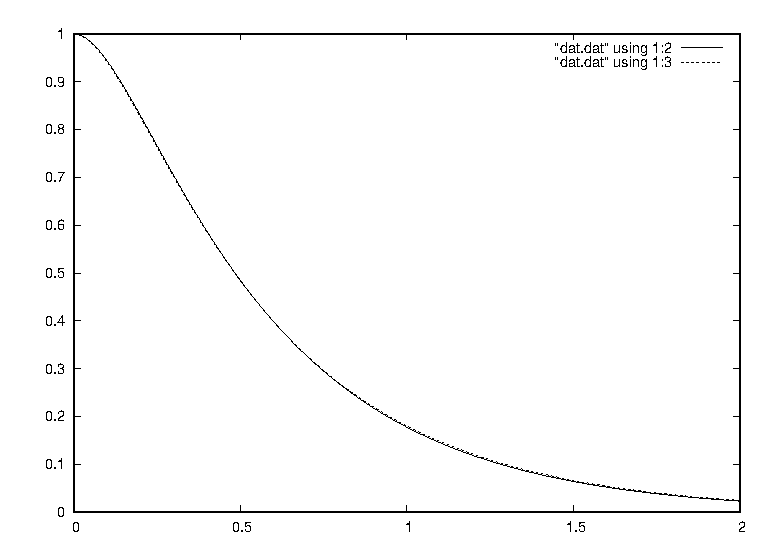
\includegraphics[width=150mm,clip]{ode1_1.eps}
	\flushright
	\vspace{-15pt}
	\caption{t-yのグラフ:厳密解と差分解($\Delta t=0.01$)}
	 \label{fig:1}
\end{figure}






%%%%%%%%%%%%%%%%%%%%%%%%%%%%%%%%%%%%%%%%%%%%%%%%%%%%%%
%		 		    本文終了		 					 %
%%%%%%%%%%%%%%%%%%%%%%%%%%%%%%%%%%%%%%%%%%%%%%%%%%%%%%

\end{document}